\begin{theorem}
Sea $\Phi \subseteq \form{S}$ un conjunto de fórmulas satisfactible ($\mbox{Sat}(\Phi)$ y T un tableau abierto para $\Phi$. ENtonces existe una rama abierta $r$ de T tal que $\mbox{Sat}(\Gamma_r)$. 
\end{theorem}
\begin{proof}
Desmotraremos que existe una interpretación $\g{Y}$ y una rama $r$ tales que $\g{Y} \models \Gamma$ e $\g{Y} \models \Phi$.
\paragraph{}
Si T es un tableau finito para $\Phi$ se ha construido en número finito de pasos
\[ \xymatrix{{T_0}\ar@{~>}[r]^{$R_1$}&{T_1}\ar@{~>}[r]^{$R_2$}&{T_2}} \ldots \xymatrix{{T_{n-1}}\ar@{~>}[r]^{$R_n$}&{T_n}}   \]
de forma que $T_0$ es un tableau inicial para $\Phi$ y $R_i$ $(1 \leq i \leq n)$ es una regla. Se hace la demostración por inducción sobre n. 
\begin{itemize}
	\item[$n=0)$] $T_0$ es un tableau inicial donde $\gamma=\{\varphi_1, \, \varphi_2, \ldots, \varphi_n \subseteq \Phi\}$. Puesto que $\mbox{Sat}(\Phi)$, tenemos que $\mbox{Sat}(\Gamma)$.
	\item[$n\geq 1)$] $\xymatrix{{T_{n-1}}\ar@{~>}[r]^{$R_n$}&{T_n}}$. La regla $R_n$ extiende una rama $r$ de $T_{n-1}$. Por otro lado hay una rama $r$ de $T_{n-1}$ tal que $\mbox{Sat}(\Gamma_r')$.
	\newpage
	\begin{itemize}
		\item Si $r \neq r'$ entonces 
		
		\begin{figure}[h!]
		\centering
		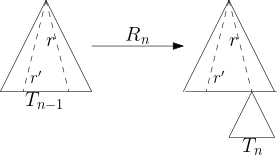
\includegraphics[width=4cm]{demo_arbo.png}
		\end{figure}
		
		$r'$ también es una rama.
\end{itemize}
	Si $R_n=R_{\mbox{hipo}}$, existe $\varphi \in \Phi$ tal que 
	
	\begin{figure}[h!]
		\centering
		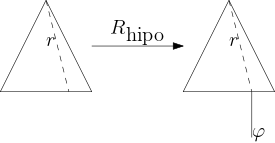
\includegraphics[width=4cm]{demo_arbo_2.png}
		\end{figure}
		
		Por hipótesis de inducción existe $\g{Y}$ tal que $\g{Y} \models \Gamma^{n-1}_r$ y $\g{Y} \models \Phi$. Puesto que $\varphi \in \Phi$, tenemos que $\g{Y} \models \varphi$ por tanto 
		\[ \g{Y} \models \Gamma^{n-1}_r \cup \{\varphi\}=\Gamma^n_r \]
		Los casos $R_n=R_\alpha$, $R_n=R_\beta$ y $R_n=R_\sigma$ son similares al caso de la lógica proposicional. 
		\paragraph{}
		$R=R_\delta$ en este caso existe $\delta \in \Gamma^{n-1}_r$ y $\Gamma^n_r=\Gamma^{n-1}_r \cup \{\delta(c)\}$. Por hipótesis de inducción existe $\mathfrak{Y}$ tal que 
		\[ \g{Y} \models \Gamma^{n-1}_r \cup \{\delta(c)\}=\Gamma^n_r \]
		En el lema anterior la única modificación entre $\g{Y}$ e $\g{Y}'$ es la constante $c$. Puesto que es auxiliar $c \not \in \mbox{voc}(\psi)$ para $\psi \in \Phi$. Por tanto $\g{Y}' \sim_{\psi} \g{Y}$ para $\psi \in \Phi$ y tenemos $\g{Y}' \models \psi$ para  $\psi \in \Phi$. Es decir
		\[  \g{Y}' \models \Phi  \]
\textit{Se dejan como ejercicio los casos $R_n=R_\gamma$ y $R_n=R_\theta$}			 
\end{itemize}
\end{proof}
\begin{Corolario}
Se tiene que
\begin{enumerate}
	\item Si $\Phi \subseteq \form{S}$ y $\Phi$ tiene un tableau cerrado, entonces $\mbox{InSat}(\Phi)$.
	\item $\tc{\Phi}{\varphi}$ entonces, $\Phi \models \varphi$.
\end{enumerate}
\end{Corolario}